\documentclass[11pt,a4paper]{article}
\usepackage{amsmath}
\usepackage{amsthm}
\usepackage{graphicx}
\usepackage[linesnumbered, ruled, vlined]{algorithm2e}
\usepackage[noend]{algpseudocode}
\usepackage{enumerate}
\usepackage{xcolor}
\usepackage{framed}
\usepackage{bm}
\usepackage{pifont}
\usepackage{multicol}
\usepackage{lipsum}
\usepackage{tikz}
\usetikzlibrary{calc}
\usepackage{array}
\usepackage{relsize}
\usepackage{comment}
\usepackage{url}
\usepackage{caption}
\usepackage{subcaption}
\usepackage{mathtools}
\usepackage{thmtools}
\usepackage{thm-restate}
\usepackage[normalem]{ulem}
\usepackage{cleveref}
\usepackage{xspace}
\usepackage{amssymb}
% ======================================================================
% Editing / collaboration
% ======================================================================

% Show diff (exactly one of this and the following pair of commands must be commented)
\newcommand{\add}[1]{\textcolor{blue}{#1}}
\newcommand{\del}[1]{\textcolor{gray}{#1}}

% Preview changes (exactly one of this and the previous pair of commands must be commented)
% \newcommand{\add}[1]{#1}
% \newcommand{\del}[1]{}

\newcommand{\replace}[2]{\del{#1}\add{#2}}

% Enable rendering of comments
% \newcommand{\guy}[1]{[\textcolor{blue}{\textbf{gg:}} {\footnotesize
% \textcolor{purple}{#1}]}}
% \newcommand{\matej}[1]{[\textcolor{blue}{\textbf{mp:}} {\footnotesize
% \textcolor{teal}{#1}]}}
% \newcommand{\marko}[1]{[\textcolor{blue}{\textbf{mv:}} {\footnotesize
% \textcolor{purple}{#1}]}}
% \newcommand{\arp}[1]{[\textcolor{blue}{\textbf{arp:}} {\footnotesize
% \textcolor{brown}{#1}]}}
% \newcommand{\jorge}[1]{[\textcolor{blue}{\textbf{js:}} {\footnotesize
% \textcolor{violet}{#1}]}}
% \newcommand{\akosh}[1]{[\textcolor{blue}{\textbf{af:}} {\footnotesize
% \textcolor{blue}{#1}]}}
% \newcommand{\cmt}[1]{[\textcolor{blue}{\textbf{CMT:}} {\footnotesize
% \textcolor{red}{#1}]}}
% \newcommand{\TODO}[1]{[{\textbf{\red{TODO:}}} {\footnotesize
% \textcolor{gray}{#1}]}}

% Disable rendering of comments.
\newcommand{\guy}[1]{}
\newcommand{\matej}[1]{}
\newcommand{\marko}[1]{}
\newcommand{\arp}[1]{}
\newcommand{\jorge}[1]{}
\newcommand{\akosh}[1]{}
\newcommand{\cmt}[1]{}
\newcommand{\TODO}[1]{}

\newcommand{\ignore}[1]{}

% ======================================================================
% Formatting macros
% ======================================================================

% Some text colors
\newcommand{\blue}[1]{{\color{blue}{#1}}}
\newcommand{\red}[1]{{\color{red}{#1}}}
\newcommand{\out}[1]{{\red{\sout{#1}}}}

\newcommand{\subnetName}[1]{\textbf{\texttt{#1}}}
\newcommand{\actorName}[1]{\texttt{#1}}
\newcommand{\dataField}[1]{\texttt{#1}}
\newcommand{\funcName}[1]{\textit{\texttt{#1}}}
\newcommand{\funcParam}[1]{\textit{#1}}
\newcommand{\accountName}[1]{\texttt{#1}}
\newcommand{\accountNameFull}[2]{\subnetName{#1}.\texttt{#2}}
\newcommand{\tx}[1]{\textit{#1}}
\newcommand{\funcNameFull}[3]{\subnetName{#1}.\actorName{#2}.\funcName{#3}}
\newcommand{\var}[1]{\textit{#1}}

\newtheorem{example}{Example}

% ======================================================================
% Macros for names to use in the text
% ======================================================================

\newcommand{\ipcFull}{Interplanetary Consensus\xspace}
\newcommand{\ipc}{IPC\xspace}
\newcommand{\sa}{\actorName{ISA}\xspace}
\newcommand{\saOf}[1]{$\sa_\subnetName{#1}$}
\newcommand{\saFull}{IPC Subnet Actor\xspace}
\newcommand{\saFulls}{IPC Subnet Actors\xspace}
\newcommand{\gw}{\actorName{IGA}\xspace}
\newcommand{\gwFull}{IPC Gateway Actor\xspace}
\newcommand{\actor}{actor\xspace} % TODO: Get rid of these and use the word "actor" directly in text. The name is very unlikely to change.
\newcommand{\actors}{actors\xspace}
\newcommand{\pofFull}{Proof of Finality\xspace}
\newcommand{\pofsFull}{Proofs of Finality\xspace}
\newcommand{\pof}{\textit{PoF}\xspace}
\newcommand{\postoffice}{postbox\xspace}

% ======================================================================
% Legacy macros
% ======================================================================

\newtheorem{claim}{Claim}
\newtheorem{notation}{Notation}
\newtheorem{invariant}{Invariant}
\newtheorem{execution}{Execution}
\newtheorem{ensemble}{Ensemble}
\newtheorem*{ensemble*}{Ensemble}
\newtheorem{strategy}{Strategy}
\newtheorem*{strategy*}{Strategy}
\newtheorem{assumption}{Assumption}
\newtheorem*{theorem*}{Theorem}

\newcommand{\alg}{$\mathcal A$}
\newcommand{\act}{\alpha}
\newcommand{\wrt}{w.r.t.\/}
\newcommand{\adv}{\sigma}
\newcommand{\SN}{\mathcal{SN}}
\newcommand{\PN}{\mathcal{PN}}
\newcommand{\parent}[1]{\texttt{parent}(#1)}
\newcommand{\user}{u}
\newcommand{\fil}{\textit{amt}\xspace}
\newcommand{\txwf}{$tx(\fil,\; \user,\; fee)$\xspace} %tx w\ fee
\newcommand{\txnf}{$tx(\fil,\; \user)$\xspace} %tx no fee
\newcommand{\chkp}{$\langle \texttt{chkp},\; fee \rangle $\xspace} %checkpoint
\newcommand{\pofs}{$pofs$\xspace}
\newcommand{\prop}{$\langle \texttt{prop},\; fee, \; dest \rangle $\xspace} 
\newcommand{\report}{$\langle \texttt{report},\; \pofs \rangle $\xspace} %report slash
\newcommand{\slashop}{$\langle \texttt{slash},\; \pofs \rangle $\xspace} %slash
\newcommand{\pUp}{\textsc{PropUp}}
\newcommand{\pDn}{\textsc{PropDn}}
\newcommand{\pHr}{\textsc{PropHere}}
\newcommand{\smr}{SMR\xspace}
\newcommand{\gov}{\textit{gov-acc}\xspace}
\newcommand{\pom}{\textit{PoM}\xspace} % Proof of Misbehavior
\newcommand{\verifyGfinal}[2]{\textit{verifyGlobalFinality}({#1},{#2})\xspace} % verify the global finality of (#1-state/tx) in the child subnet with assitance of (#2-proof).
\newcommand{\verifyPfinal}[2]{\textit{verifyParentFinality}({#1},{#2})\xspace} % verify the global finality of (#1-state/tx) in the parent subnet with assitance of (#2-proof).
\newcommand{\ssc}{\textit{ShouldSubmitCheckpoint}\xspace}
\newcommand{\prf}{\textit{PoF}\xspace}
\newcommand{\data}{\textit{data}\xspace}
\newcommand{\dest}{\textit{dest}\xspace}
\newcommand{\src}{\textit{src}\xspace}
\newcommand{\bqueue}{bottom-up registry\xspace}
\newcommand{\tqueue}{top-down registry\xspace}  
\newcommand{\tcheckpoint}{top-down checkpoint\xspace}
\newcommand{\eoa}{\textit{EOA}\xspace}
\newcommand{\propagate}{\textit{propagate}}
\newcommand\T[1]{\noindent\textbf{#1}}
\newcommand{\impl}{IPC reference implementation\xspace} % name it differently?

% \let\period.
% \catcode`\.\active 
% \def\uppercasesingleletter#1{\uppercase{#1}}
% \def.{\period\afterassignment\periodx\let\next= }
% \def \periodx{\ifcat\space\next \next\expandafter\uppercasesingleletter \else\expandafter\next\fi}


% \usepackage{caption}
% \usepackage{subcaption}
% \usepackage[utf8]{inputenc}
% \usepackage{xcolor}
% \usepackage[linesnumbered, ruled, vlined]{algorithm2e}
% %\usepackage{amssymb}
% \usepackage{amsmath}
% \usepackage{nccmath}
% \usepackage{amsthm}
% \usepackage{thmtools}
% \usepackage{thm-restate}
% \usepackage{hyperref}
% \usepackage[capitalise]{cleveref}
% \usepackage[normalem]{ulem}
% \usepackage{mathtools}
% \usepackage{empheq}
% \usepackage{fontawesome}
% \usepackage{graphicx}
% \usepackage{bm}
% \usepackage{threeparttable}

% \newtheorem{theorem}{Theorem}
% \newtheorem{corollary}{Corollary}
% \newtheorem{lemma}{Lemma}
% \newtheorem{definition}{Definition}

% \def\cameraReady{} % set to true
% \let\cameraReady\undefined % set to false

% \newcommand{\vcsig}{vc_{\textit{sig}}}
% \newcommand{\PoApush}[1]{\texttt{PoA\_push}(#1)}
% \newcommand{\PoAcommit}[1]{\texttt{PoA\_commit}(#1)}
% \newcommand{\PoApull}[1]{\texttt{PoA\_pull}(#1)}
% \newcommand{\PoAdeliver}[1]{\texttt{PoA\_deliver}(#1)}
% \newcommand{\Prove}{\texttt{CreateProof}}
% \newcommand{\Verify}{\texttt{Verify}}
% \newcommand{\InTransit}{\textit{InTransit}}
% \newcommand{\NewInTransit}{\textit{NewInTransit}}
% \newcommand{\reconstruct}{\text{RECONSTRUCT}}
% \newcommand{\pull}{\text{PULL}}
% \newcommand{\CV}{\text{CodedVector}}
% \newcommand{\poa}{\text{PoA}}
% \newcommand{\msg}{\textit{msg}}
% \newcommand{\PoAR}{\text{PoA\&R}}

% \newcommand{\setS}{{\mathcal S}} 
% \newcommand{\setX}[1]{{\mathcal X}_{#1}}
% \newcommand{\setY}[1]{{\mathcal Y}_{#1}}
% \newcommand{\currTime}{\textit{currTime}}

% \newcommand{\gray}[1]{\textcolor{gray}{#1}}
% \newcommand{\red}[1]{\textcolor{red}{#1}}
% \newcommand{\blue}[1]{\textcolor{blue}{#1}}
% \newcommand{\purple}[1]{\textcolor{purple}{#1}}
% \newcommand{\magenta}[1]{\textcolor{magenta}{#1}}
% \newcommand{\green}[1]{\textcolor{green}{#1}}
% \newcommand{\guy}[1]{{\footnotesize{\color{blue} [Guy: #1]}}}
% \newcommand{\shir}[1]{{\footnotesize{\color{red} [Shir: #1]}}}
% \newcommand{\sasha}[1]{{\footnotesize{\color{green} [Sasha: #1]}}}
% \newcommand{\alberto}[1]{{\footnotesize{\color{magenta} [Alberto: #1]}}}
% \newcommand{\lef}[1]{{\footnotesize{\color{red} [Lef: #1]}}}
% % \newcommand{\ynew}[1]{\magenta{#1}}
% % \newcommand{\gnew}[1]{\blue{#1}}
% % \newcommand{\gold}[1]{\blue{\sout{#1}}}
% % \newcommand{\out}[1]{\red{\sout{#1}}}

% %========================
% %  Math
% %========================

% \newcommand{\sysname}{Layered-SMR\xspace}

% \newcommand{\para}[1]{\left( #1 \right)}  %Shortcuts in equations for parentheses
% \newcommand{\brac}[1]{\left\{ #1 \right\}}
% \newcommand{\sbrac}[1]{\left[ #1 \right]}
% \newcommand{\floor}[1]{\left\lfloor #1 \right\rfloor}
% \newcommand{\ceil}[1]{\left\lceil #1 \right\rceil}
% \newcommand{\norm}[1]{\left\Vert#1\right\Vert}
% \newcommand{\abs}[1]{\left\vert#1\right\vert}
% \newcommand{\reals}{\mathbb{R}}
% \newcommand{\rationals}{\mathbb{Q}}
% \newcommand{\integers}{\mathbb{Z}}
% \newcommand{\naturals}{\mathbb{N}}
% \newcommand{\Proc}{\Pi}
% \newcommand{\Expectation}{\mathbb{E}}

% \newcommand{\eps}{\varepsilon}

% \newcommand{\TT}[1]{\noindent\textbf{#1}}
% \newcommand{\I}[1]{\smallskip\noindent\textit{#1}}
% \newcommand{\II}[1]{\noindent\textit{#1}}
% \newcommand{\bp}[1]{\Big(#1\Big)}
% %\newcommand{\given}[1]{\,\Big\vert\,#1}


% \providecommand{\ie}{\emph{i.e.,} }
% \providecommand{\eg}{\emph{e.g.,} }


% \DeclareMathOperator{\E}{\mathbb{E}}


%%%%%%%%%%%%%%%%%%%%%%%%%%%%%%%%%%%%%%%%%%%%%%%%%%%%%%
%%%%%%%%%%%%%%%%%%%%%%%%%%%%%%%%%%%%%%%%%%%%%%%%%%%%%%
%%%%%%%%%%%%%%%%%%%%%%%%%%%%%%%%%%%%%%%%%%%%%%%%%%%%%%
%%%%%%%%%%%%%%%%%%%%%%%%%%%%%%%%%%%%%%%%%%%%%%%%%%%%%%
%%%%%%%%%%%%%%%%%%%%%%%%%%%%%%%%%%%%%%%%%%%%%%%%%%%%%%
%%%%%%%%%%%%%%%%%%%%%%%%%%%%%%%%%%%%%%%%%%%%%%%%%%%%%%
%%%%%%%%%%%%%%%%%%%%%%%%%%%%%%%%%%%%%%%%%%%%%%%%%%%%%%
%%%%%%%%%%%%%%%%%%%%%%%%%%%%%%%%%%%%%%%%%%%%%%%%%%%%%%
%%%%%%%%%%%%%%%%%%%%%%%%%%%%%%%%%%%%%%%%%%%%%%%%%%%%%%
%%%%%%%%%%%%%%%%%%%%%%%%%%%%%%%%%%%%%%%%%%%%%%%%%%%%%%



\graphicspath{{figs/}}
\newcounter{myCounter}

\begin{document}



\title{\nameFull (\nameAbbr)}
\date{}
\author{Consensus Lab}
% \authornote{Both authors contributed equally to this research.}
% \orcid{1234-5678-9012}
% \author{G.K.M. Tobin}
% \authornotemark[1]
%\email{sgoren@campus.technion.ac.il}
% \orcid{https://orcid.org/0000-0003-2158-161X}
% \affiliation{%
%     \institution{Technion}
%     \country{Israel}
%     }

\maketitle
\begin{abstract}
TODO
\end{abstract}

% ----------------------------------------------------------------
% ----------------------------------------------------------------

\section{Introduction}
\label{sec:introduction}

A blockchain system is a platform for hosting replicated applications (represented by smart contracts in Ethereum [??] or actors in Filecoin [??]).
A single system can, at the same time, host many such applications,
each of which containing logic for processing inputs (also known as transactions, requests, or messages) and updating its internal state accordingly.
The blockchain system stores multiple copies of those applications' state and executes the associated logic.
In practice, applications are largely (or even completely) independent.
This means that the execution of one application's transactions rarely (or even never) requires accessing the state of another application.

Nevertheless, most of today's blockchain systems process all transactions for all hosted applications (at least logically) sequentially.
The whole system maintains a single totally ordered transaction log containing an interleaving of the transactions associated with all hosted applications.
The total transaction throughput the blockchain system can handle thus must be shared by all applications, even completely independent ones.
This may greatly impair the performance of such a system at scale (in terms of the number of applications).
Moreover, if processing a transaction incurs a cost (transaction fee) for the user submitting it, using the system tends to become more expensive when the system is saturated.

The typical application hosted by blockchain systems is asset transfer between users (wallets).
Asset transfers often involve other applications and may create system-wide dependencies between different parts of the system state.
In general, if users interacted in an arbitrary manner (or even uniformly at random), this would indeed be the case.
However, in practical systems, users tend to cluster in a way that those inside a cluster interact more frequently than users from different clusters.
While this ``locality" makes it unnecessary to totally order transactions confined to different clusters (in practice, the vast majority of them),
many current blockchain systems spend valuable resources on doing so anyway.

An additional issue of such systems is the lack of flexibility in catering for the different hosted applications.
Different applications may prefer vastly different trade-offs (in terms of latency, throughput, security, durability, etc...).
For example, a high-level money settlement application may require the highest levels of security and durability, but may more easily compromise on performance in terms of transaction latency and throughput.
On the other hand, one can imagine a distributed online chess platform (especially one supporting fast chess variants) whose state is mostly ephemeral (lasting until the end of the game) but which requires high throughput (for many concurrent games) and low latency (few people like waiting 10 minutes for the opponent's move).
While the former is an ideal use case for the Bitcoin network, the latter would probably benefit more from being deployed in a single data center.
\jorge{It's an okay example but just noting that concurrent games are independent and can be seen as different applications; I don't think it negates the specific point being made here.}

In the above example, one can also easily imagine those two applications being mostly, but not completely independent.
E.g., a chess player may be able to win some money in a chess tournament and later use it to buy some goods outside of the scope of the chess platform.
In such a case, few transactions involve both applications (e.g., paying the tournament registration fee and withdrawing the prize money).
The rest (e.g., the individual chess moves) are confined to the chess application and can thus be performed much faster and much cheaper (imagine playing chess by posting each move on Bitcoin for comparison).

\ipcFull (\ipc) is a system that enables the deployment of heterogeneous applications on heterogeneous underlying blockchain platforms, while still allowing them to interact in a secure way.
The basic idea behind \ipc is dynamically deploying separate, loosely coupled blockchain systems that we call \emph{subnets}, to host different (sets of) applications.
Each subnet runs its own consensus protocol and maintains its own ordered transaction log.

\ipc is organized in a hierarchical fashion, where each subnet, except for one that we call the \emph{rootnet}, is associated with exactly one other subnet called its \emph{parent}.
Conversely, one parent can have arbitrarily many subnets, called \emph{children}, associated with it.

This tree of subnets expresses a hierarchy of trust.
All components of a subnet and all users using it are assumed to fully trust their parent and regard it as the ultimate source of truth.
Note that, in general, trust in all components of the parent subnet is not required, but the parent system as a whole is always assumed to be correct (for some definition of correctness specific to the parent subnet) by its child.

To facilitate the interaction between different subnets, \ipc provides mechanisms for inter-subnet communication.
Since subnets are distributed transaction-processing systems
without an obvious single entity to submit transactions to one subnet on behalf of another subnet,
we introduce processes called \emph{\ipc agents} that read the replicated state of one subnet and submit transactions on its behalf to another subnet.
Participants running those \ipc agents get rewarded for such mediation.
Out of the box, \ipc provides several primitives for subnet interaction, such as
\begin{enumerate}
    \item Transfer of funds between accounts residing in different subnets.
    \item Saving checkpoints (snapshots) of a child subnet's replicated state in the replicated state of its parent.
    \item Submitting transactions to a subnet by the application logic of another subnet.
\end{enumerate}

The operating model described above is simple but powerful.
In particular, it enables
\begin{itemize}
    \item Scaling, by using multiple blockchain/SMR platforms to host a large number of applications.
    \item Optimization of blockchain platforms for applications running on top of them.
    \item Governance of a child subnet by its parent, by way of the parent serving as the source of truth for the child and, for example, maintaining the child's configuration, replica set, and other subnet-specific data.
    \item ``Inheriting" by the subnet of some of its parent's security and trustworthiness, by periodically anchoring its state in the state of the parent using checkpoints.
\end{itemize}

In the rest of this document, we describe \ipc in detail.
In \cref{sec:preliminaries} we define...
\TODO{Finish this when all sections are stable.}
\section{Model}
\label{sec:model}

The vocabulary used throughout this document is summarized in the IPC Glossary \cite{glossary}.
The reader is encouraged to read the IPC Glossary before continuing.

\matej{When the Glossary becomes stable, we can maybe add it as an appendix to this document.}

\subsection{Computation and failure model}

We model \ipc as a distributed (``message-passing") system consisting of \emph{processes} that communicate by exchanging \emph{messages}%
\footnote{Network messages are not to be confused with Filecoin actor messages, that this document refers to as transactions.}
over a network. 
In practice, a process is a program running on a computer, having some state, and reacting to external events and messages received over a communication network.
We describe processes as exemplified in \Cref{alg:process-definition}.

\begin{algorithm}[H]
\footnotesize
\caption{Process definition.}\label{alg:process-definition}
  \DontPrintSemicolon
  \SetKwProg{Component}{$\blacktriangleright$ \bf}{:}{\KwRet}
  \SetKwFor{UponKW}{upon}{do}{fintq}
  \SetKw{Trigger}{trigger}
  variable = initial value\\
  variable = initial value\\
  ...\\
  \Component{process}{
     \UponKW{event(params...)}{
       \tcp{Logic to execute atomically}
     }
     \UponKW{message(params...)}{
       \tcp{Logic to execute atomically}
     }
     ...
}
\end{algorithm}

A process that performs all the steps exactly as prescribed by the protocols it is participating in is \emph{correct}.
A process that stops performing any steps (i.e., \emph{crashes}) or that deviates from the prescribed protocols in any way is \emph{faulty}.
If a process is correct or may only fail by crashing, it is \emph{benign}.
A non-benign process is \emph{malicious}.
\matej{We can remove terms we end up not using...}

In general, faulty processes can be malicious (Byzantine), i.e., we do not put any restrictions on their behavior, except being computationally bounded and thus not being able to subvert standard cryptographic primitives, such as forging signatures or inverting secure hash functions.
If the implementation of some component in our design requires additional assumptions on the behavior of faulty processes, they will be stated explicitly.
% We do not make a general statement about the fault tolerance of \ipc as a system, as to how many faulty processes the system can sustain.
% This depends on the final implementation of its components.

We use the term \emph{participant} to describe an entity participating in the system that controls one or more processes.
All processes controlled by one participant are assumed to be in the same trust domain -- they trust each other, i.e., assume each other's correctness.
For example, a participant in the child subnet will probably run multiple processes:
one for participating in the child subnet's protocol (child replica),
one for participating in the parent subnet (parent replica),
and one process that processes the information from the above two and submits transactions accordingly (\ipc agent).
We precisely define the replicas and the \ipc agent (all of them being processes) in \Cref{sec:components,sec:smr}.
The \ipc agent of a participant always assumes that the information it receives from "its own" child replica is correct.
However, messages received from another participant's replica or \ipc agent are seen as potentially malicious.

The synchrony assumptions may vary between different components of \ipc.
We thus state those assumptions whenever necessary, when describing concrete implementations of \ipc components.

\subsection{State machine replication (SMR) and \dapps}
\label{sec:smr}

\paragraph{SMR and replicated state.}
A \emph{state machine replication (SMR) system}%
\footnote{In this document, we use the terms ``SMR system" and ``blockchain" interchangeably.}
is a system consisting of processes called \emph{replicas}, each of which locally stores a copy of (or at least has access to) \emph{replicated state}
that it updates over time by applying a sequence of \emph{transactions} to it.
Without specifying the details of it, we assume that any process can \emph{submit} a transaction to an SMR system (we call such a process an \emph{SMR client})
and that this transaction will eventually be ordered and applied to the replicated state.
We call an SMR system that is part of \ipc a \emph{subnet}.

An SMR system guarantees to each correct replica that, after applying $n$ transactions to its local copy of the replicated state,
the latter will be identical to any other correct replica’s copy of the replicated state after applying $n$ transactions.
The replicas achieve this by executing an \emph{ordering protocol} to agree on a common sequence of transactions to apply to the replicated state.

Note that replicas do not necessarily all hold the same replicated state at any instant of real time,
since each replica might be processing transactions at a different time.
In this context, there is no such thing as “the current replicated state of the SMR system”.
There is only the current replicated state of a single replica.
The replicated state of the system is only an abstract, logical construct
useful for reasoning about transitions from one replicated state to another,
happening at individual replicas by applying transactions (at different real times).
When referring to a “current” replicated state, we mean the state resulting from the application of a certain number of transactions to the initial state.

\paragraph{Smart contracts.}
The replicated state of an SMR system can be logically subdivided into multiple \emph{\dapps} (a.k.a. actors in Filecoin).
A \dapp is a portion of the replicated state with well-defined semantics.
It defines the logic (e.g., expressed in a programming language, like Solidity in Ethereum)
that a replica needs to execute when applying transactions and the new state that results from it.

We model a \dapp as a logical object in the replicated state that contains arbitrary variables representing its state.
Its associated logic reacts to \emph{events} triggered by (1) the application of transactions or (2) execution of other (or even own) smart contract logic. We describe smart contracts as exemplified in \Cref{alg:dapp-definition}.

\begin{algorithm}[H]
\footnotesize
\caption{\dapp definition}\label{alg:dapp-definition}
  \DontPrintSemicolon
  \SetKwProg{Component}{$\blacktriangleright$ \bf}{:}{\KwRet}
  \SetKwFor{UponKW}{upon}{do}{fintq}
  \SetKw{Trigger}{trigger}
  variable = initial value\\
  variable = initial value\\
  ...\\
  \Component{\dapp name}{
     \UponKW{event(params...)}{
       \tcp{Logic to execute}
       \Trigger event(params...)
     }
     \UponKW{tx(params...)}{
       \tcp{Logic to execute}
       \Trigger event(params...)
     }
     ...
}
\end{algorithm}
Note that, despite using similar syntax to describe processes and \dapps, those are fundamentally different.
The former usually represent OS-level processes running on some physical machine,
the latter are an abstraction over the replicated state of an SMR system and their logic is being executed by all its replicas.
While a process can submit a transaction to an SMR system, a \dapp cannot.

\paragraph{Interaction between subnets.}
In \ipc, whole subnets need to interact, i.e., the replicated state of one subnet must react to (changes in) the replicated state of another subnet.
As the replicated state of every subnet is distributed among its replicas and evolves independently of other subnets,
we must establish a mechanism for interactions between the states of subnets.
In particular, we must explicitly link the two replicated states of two subnets.
More precisely, for any interaction between two subnets ($A$ and $B$), define block heights $h_A$ and $h_B$,
such that $A$'s replicated state at height $h_A$ considers $B$'s replicated state to have evolved exactly until $h_B$.

\paragraph{\PofsFull.}To this end, we define a \emph{\pofFull (\pof)} to be data that proves that an SMR system definitively reached a certain replicated state.
Regardless of the SMR system's ordering protocol's approach to finality (e.g., immediate finality for classic BFT protocols, or probabilistic finality in PoW-based systems),
a \pof convinces the the proof's verifier that the replicated state the \pof refers to will not be rolled back.
For example, for a BFT-based SMR system, a quorum of signatures produced by its replicas can constitute a \pof.
We denote by \emph{\pof(tx)} the proof that an SMR system reached a state in which transaction \emph{tx} already has been applied.



\subsection{Money}

For each pair of subnets in a parent-child relationship, we assume that there exists a notion of \emph{money} (measured in \emph{coins}) common to both subnets.%
\footnote{One can easily generalize the design to decouple the use of money between a parent and its child, but we stick with using the same kind of money in both subnets for simplicity.}
Each end user of the SMR system is assumed to have a personal wallet and a corresponding account in some subnet.

We also assume that the submission, ordering, and applications of transactions is associated with a monetary cost.
Each SMR client submitting a transaction to a subnet is assumed to have an account in that subnet, from which this cost is deducted.
If the funds are insufficient, the SMR system ignores the transaction.
 % - Components and their Interfaces
 %   - Parent subnet node
 %   - Child subnet node
 %   - IPC module
 %   - Subnet actor
 \section{Components and their Interfaces}
 \label{sec:components}

In \ipc, whole subnets need to interact.
I.e., the replicated state of one subnet must react to (changes in) the replicated state of another subnet.
As the replicated state of every subnet is distributed among its replicas and evolves independently of other subnets,
we must establish a mechanism for interactions between the states of subnets.
In particular, we must explicitly link the two replicated states of two subnets.
More precisely, for any interaction between two subnets ($A$ and $B$), define block heights $h_A$ and $h_B$,
such that $A$'s replicated state at height $h_A$ considers $B$'s replicated state to have evolved exactly until $h_B$.

To this end, we define a \emph{\pofFull (\pof)} to be data that proves that an SMR system definitively reached a certain replicated state.
Regardless of the SMR system's ordering protocol's approach to finality (e.g., immediate finality for classic BFT protocols, or probabilistic finality in PoW-based systems),
a \pof convinces the the proof's verifier that the replicated state it refers to will not be rolled back.
We denote by \emph{\pof(tx)} the proof that an SMR system reached a state in which transaction \emph{tx} already has been applied.
For example, for a BFT-based SMR system, a quorum of signatures produced by its replicas can constitute a \pof.



We separate the software needed to run \ipc into three processes and two \dapps:

\matej{\todo{Express those components and their interfaces also in pseudocode.}}
\begin{enumerate}
    \item \textbf{\ipc agent:} The software that is in charge of the interactions between the two blockchains. This includes, for example, observers for the parent and child subnets. (Note that it is a process and not a smart contract). The \ipc agent is a piece of software that mediates the interactions between the child and parent \smr software modules.    
    \item \textbf{Parent \smr replica:} The software that runs the parent blockchain. Note that this module also entails the interaction with the \ipc smart contract~\sa, which is maintained at the parent subnet. Any update that the parent process performs on \sa is notified to the \ipc agent.
    \item \textbf{Child \smr replica:} The software that runs the child blockchain. Note that some of the rules the child blockchain must satisfy are listed in~\sa. Any output operation (withdraw, checkpoint) is notified to the parent process through the \ipc agent. 
%    \item \textbf{IPC smart contract / subnet actor (\sa):} The smart contract implementation that is running on the parent blockchain. It is invoked only through transactions that are included in the parent blockchain.
    \item \textbf{IPC subnet actor (\sa):} The smart contract implementation that is running on the parent blockchain. It is invoked only through transactions that are included in the parent blockchain.
    \item \textbf{IPC coordinator/gateway actor (\gw):} a smart contract that exists in every non-leaf subnet in the \ipc hierarchy and contains methods facilitating inter-subnet operations.	
\end{enumerate}


We now define minimal interfaces between the different modules that enable the correct operation of an \ipcFull system.
A guiding principle in the interface design is to minimize changes to the \smr codebase; therefore, most extra logic of the \ipc will be added into the \ipc agent and the smart contracts \sa~and~\gw. Doing so should facilitate the deployment of \ipc with new \smr protocols by not requiring a developer familiar with \ipc to be an expert on \smr: some understanding is still needed to optimize the agent's implementation, but the \smr code would remain portable.

We require four interfaces: (i) \ipc agent --- parent \smr, (ii) \ipc agent --- child \smr, (iii) parent \smr --- \sa, and (iv) any \smr --- \gw. Both (i) and (ii) can comprise of only:
\begin{enumerate}
    \item Agent submits a transaction~\tx to the \smr process.%
    \footnote{As part of the notification defined below, it could be that after submitting \tx, until the \smr process returns \textit{complete} (perhaps with a finality parameter) or \textit{declined}, \tx is considered \textit{pending}.}
    \item Agent queries the state of the \smr process. The \smr process returns its current state (possibly limited to only a requested part of the state).
    \item \smr process notifies the agent on events of interest (e.g., changes to the state of~\sa).
\end{enumerate}

The interface between an \smr and~\sa or~\gw is based on the execution engine of that \smr and the functionality desired by~\sa. The specifics of the execution engine's system calls depend on implementation. Whenever such a call is not clear from context we provide a description of what it entails. \\


\T{The state of \sa includes representations of:}
% accounting
% Consensus functionality
% functionalities: proofOfFinality
\begin{itemize}
    \item Accounting data. This can vary from a single account representing all the parent's coins in the child to an account balance for each user in the child subnet (custodial vs non-custodial accounting). We continue with the non-custodial approach as the other can be viewed as a specific limitation of it.
    %
    \item Governance account (denoted \gov). This account facilitates the economic design of a subnet. It can be used for governing operations of the subnet. For example, collecting fees and making payments (to validators, for checkpoint reimbursement etc.) 
    %
    \item Consensus information. The data (or a pointer to it) that is needed to run the ordering of the subnet.
    \begin{itemize}
        \item Consensus protocol.
        \item Subnet configuration such as the validator set, voting rights, collateral deposits, etc.
        \item Payments methods for participation. E.g., transaction fee mechanism, block rewards.
    \end{itemize}
    %
    \item Finality verification. A method to Verify that a state/\tx is final%
    \footnote{Finality is an elusive concept that we do not take upon ourselves to define here. For simplicity, we assume finality in a Boolean manner, either \tx is final or it is not. This could easily be generalized to parameterized finality of the sort ``the probability of \tx persisting is at least~$x$."}
    in the child subnet. For this, we will use the function \sa.\verifyGfinal{\tx}{\prf} which excepts as arguments a transaction (or state) and a \prf, and outputs True if \tx is considered globally final in the child subnet and False otherwise. This function must only depend on its inputs and the internal state of~\sa. For example, \prf is a threshold signature that can be verified against the set of validators in~\sa.
  \item Parent's finality verification. A method to verify that a state/\tx is final in the parent subnet. For this, we will use the function \gw.\verifyPfinal{\tx}{\prf} which excepts as arguments a transaction (or state) and a \prf, and outputs True if \tx is considered globally final in the parent subnet and False otherwise. This function must only depend on its inputs (and perhaps some internal state of~\gw). \arp{subnet specific, not necessarily the same method for all child subnets. Lives at the SA (needed for deposits but deposits should not depend on \gw)}
\end{itemize}
%
The above suffices for an \ipcFull system with a minimal inter-subnet functionality of users' asset-transfer, and a general \smr per subnet. We continue with the additional state required for enhanced functionalities.
%
\begin{itemize}
    \item Slashing functionality.
    \begin{itemize}
        \item List of slashable misbehaviors and a proving methodology. That is, for each slashable misbehavior there is a definition of what constitutes a valid proof of misbehavior (\pom).
        \item Incentives design, i.e., specified penalties for misbehavior and rewards for reporting.
    \end{itemize}
    %
    \item Checkpointing rules.
    \begin{itemize}
        \item When checkpoints are valid. E.g., every~$\Delta$ subnet-blocks from the previous checkpoint, or the checkpoint's $L_2$ distance from the previous is larger than~$L$.
        \item Fee payments for checkpoints.
    \end{itemize}
    %
%    \item Inter-subnet transactions service (denoted \postoffice). 
%    \sa contains functionality that can be used to transfer data from one subnet to another. In particular, consider the following case involving a smart contract.%
%    \footnote{When inter-subnet data transfer happens between users (Externally Owned Accounts --- \eoa --- in Ethereum's jargon), they can actively participate in the propagation via the \ipc agent that communicates with both the parent and child subnets. Smart contracts, on the other hand, do not have that power and, therefore, cannot communicate inter-subnets as efficiently as users (\eoa).}
%    Smart contract $\textit{SmCt}$ emits an event~$e$ that contains $\textit{data}$ which is desired to reach the destination~\textit{dest} in a different subnet.
%    The \postoffice specifies the methods and the state locations that are used by this service.
\end{itemize}
Recall that \sa lives at the parent \smr. However, some of the objects that are represented in \sa are modified in the child subnet (e.g., accounting data). Therefore, such objects are likely to have a representation in the child \smr as well.
Moreover, the representation in the child \smr may differ from those in~\sa. This is due to \sa being less frequently updated (it is part of the parent \smr state). The representations are periodically synchronized, e.g., at a checkpoint event. \Cref{fig:interfaces} illustrates the components and their interfaces.\\


% We remark that all of the above are likely to have representations in the child \smr as well. Moreover, the representation in the child \smr may differ from those in~\sa. This is due to \sa being less frequently updated (it is part of the parent \smr state). The representations are periodically synchronized, e.g., at a checkpoint event. \Cref{fig:interfaces} illustrates the components and their interfaces.
\begin{figure}[h]
     \centering
     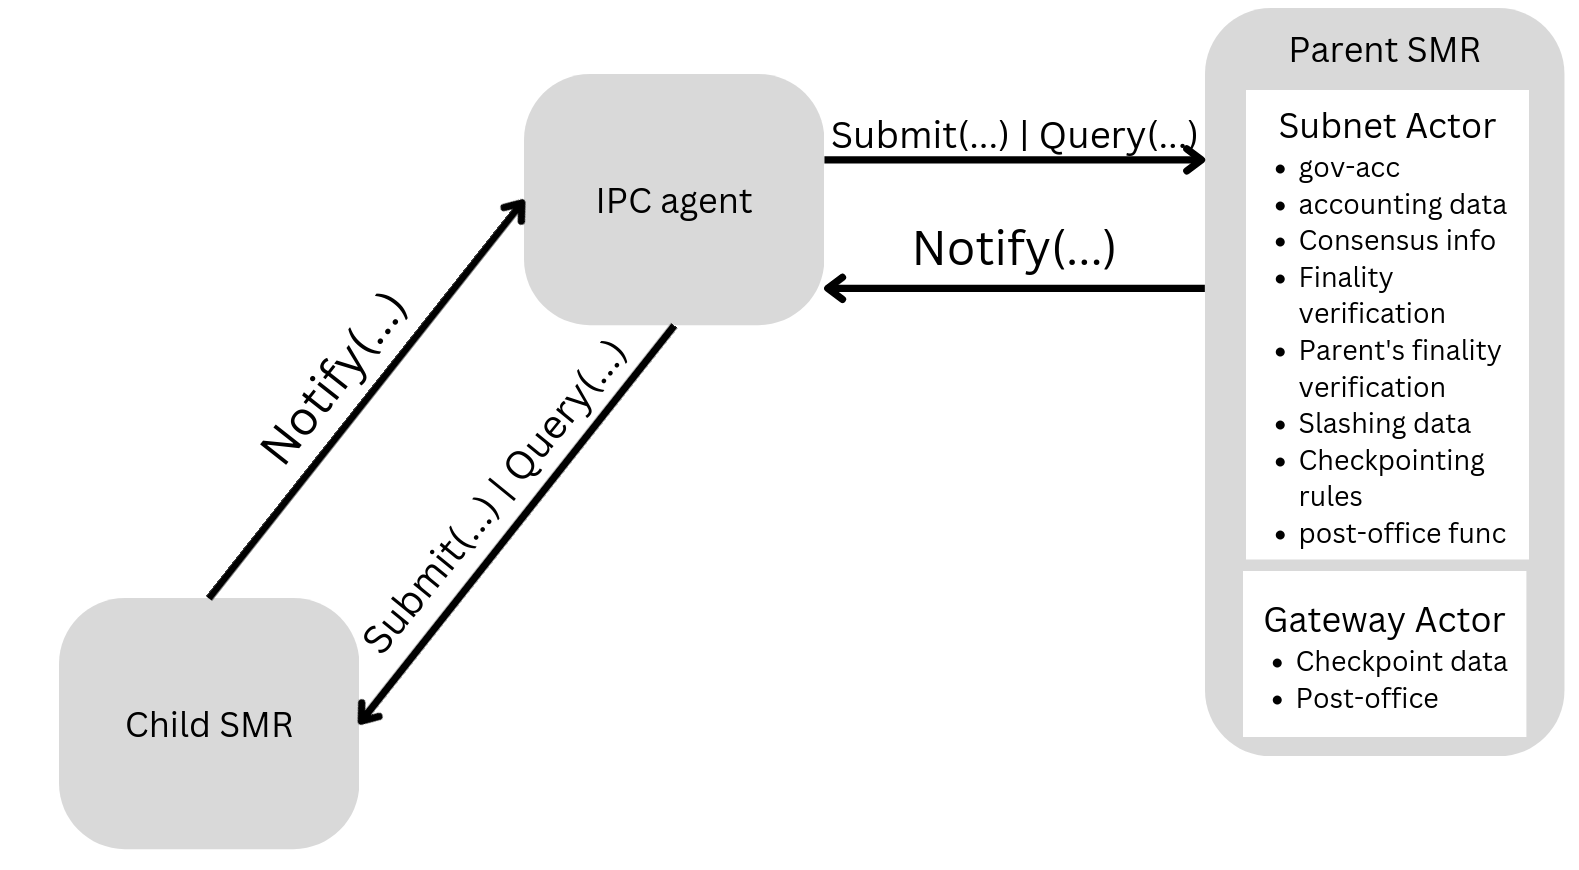
\includegraphics[width=0.75\textwidth]{compsintfs}
     \caption{The basic components and their interfaces.}
     \label{fig:interfaces}
 \end{figure}


\T{The state of \gw includes:}
\begin{itemize}
    \item Checkpoint data. The parent stores at the \gw each of the checkpoints from each direct child of it.
    \item Inter-subnet transactions service (denoted \postoffice). 
    \gw contains a registry of subnets and a functionality that can be used to transfer data from one subnet to another. 
    The \postoffice specifies the methods and the state locations that are used for these services.
    In particular, consider the following case involving a smart contract.%
    \footnote{When inter-subnet data transfer happens between users (Externally Owned Accounts --- \eoa --- in Ethereum's jargon), they can actively participate in the propagation via the \ipc agent that communicates with both the parent and child subnets. Smart contracts, on the other hand, do not have that power and, therefore, cannot communicate inter-subnets as efficiently as users (\eoa).}
    Smart contract $\textit{SmCt}$ emits an event~$e$ that contains $\textit{data}$ which is desired to reach the destination~\textit{dest} in a different subnet.
\end{itemize}
 
 
 
 % - IPC Functionality
 %  - Minimum required per subnet
 %    - Withdrawal/Deposits Interfaces
 %    - Other Operations? (Propagate?)
 %  - Enhancements
 %    - Checkpointing interfaces
 %    - Propagate
 %    - Reporting/Slashing interfaces
 %    - Atomic execution/swap, IBC-like bridges
 %  - Future stuff (google docs?)
 %    - Withdrawal at ancestor (skip parent(s)) (with timeout) etc.
\section{IPC functionality}
\label{sec:functionality}
We list in this section the functionality that should be provided by the IPC components. We first list the minimal functionality required for every subnet (deposits and withdrawals), to then extend it with enhanced functionalities. We model components as processes that produce and consume events. Events consumed by the IPC agent are the result of either a notification from one of the SMRs or the response of a query made by the IPC agent. Events produced by the IPC agent result in the IPC agent submitting a transaction that will change the state of the SMR that consumes the event.

We note that our focus is on the core functionalities, disregarding optimizations for the moment. Batching is a prime example of this. It is expected that batching will be a key optimization whenever \verifyGfinal{\tx}{\prf} is used, as calling \verifyGfinal{\tx}{\prf} can be costly. Batching allows us to perform multiple operations for one \verifyGfinal{\tx}{\prf} call, reducing its overall cost.

\subsection{Minimal Functionality}
\label{sec:minFunc}
We show in this section the functionalities for deposits and withdrawals.

\subsubsection{Deposits}
\label{sec:deposit}

\arp{Consider need to pause/remedy subnet after deposit (e.g. collateral not enough with new supply). IPC agent should check in that case}\\

A deposit is a transfer of funds (of some amount \fil) from user $\user_P$'s wallet in the parent subnet to user $u_C$'s wallet in the child subnet.
We assume that $u_P$ is a participant running a parent replica, a child replica, and an \ipc agent.%
\footnote{If $u_P$ does not run these processes, $u_P$ contacts a trusted participant that does and that performs the deposit on $u_P$'s behalf.}
The deposit is performed by the user controlling the \ipc agent as follows:
\begin{enumerate}
    \item The local \ipc agent submits to the parent \smr replica the corresponding (properly signed) transaction
    $\tx=\textit{Deposit}\left( \src, \fil, \sa.\textit{accounts}.\dest \right)$ with $\src=\user_P$ and $\dest = \user_C$.
    \item The parent SMR system orders and executes the Deposit transaction (provided $u_P$ has enough funds) by transferring $amt$ from $u_P$'s parent account to the \sa (concretely, to $u_P$'s account representation within the \sa). This effectively locks the funds within the \sa \dapp, until the \sa \dapp transfers it back to $u_P$'s account during withdrawal (see \Cref{sec:withdraw}).
    \item When the parent's replicated state that includes the transaction becomes final (for some SMR-system-specific definition of finality), the local parent replica notifies the local \ipc agent, potentially attaching a proof of finality of $PoF(tx)$ to the notification.%
    \footnote{The exact content of $PoF(tx)$ depends on the implementations of the SMR systems. It might contain, for example, a quorum of replica signatures, a Merkle proof of inclusion, or even be empty.}
    \item The \ipc agent constructs a transaction $\tx' = \textit{Deposited}\left(\langle  \src, \fil, \sa.\textit{accounts}.\dest \rangle, \prf \right)$ and submits it to the child SMR system.
    \item Upon ordering $tx'$, the replicated logic of the child SMR system mints \fil new coins and adds them to $\user_C$'s account.
\end{enumerate}

We show in \Cref{fig:deposit} the events being produced and consumed by the deposit functionality and in Algorithm~\ref{alg:deposit} the pseudocode per component to implement the functionality.

\begin{figure}[h]
     \centering
     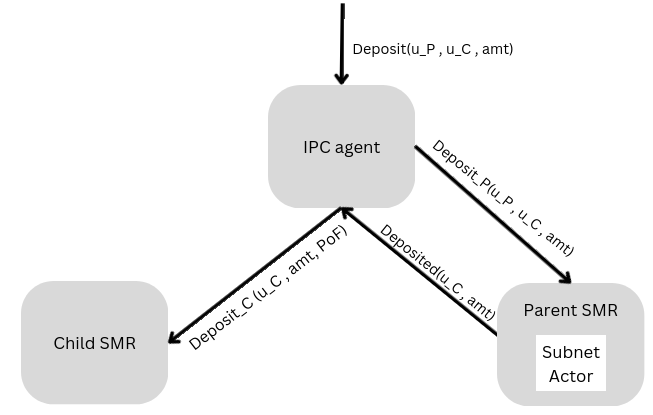
\includegraphics[width=\textwidth]{deposit}
     \caption{Events produced and consumed during a deposit.}
     \label{fig:deposit}
\end{figure}
 

\begin{algorithm}[H]
\footnotesize
\caption{Deposit operation}\label{alg:deposit}
  \DontPrintSemicolon
  \SetKwFunction{FMain}{Global}
  \SetKwProg{Pn}{Function}{:}{\KwRet}
  \SetKwInOut{Input}{input}
  \SetKwProg{Component}{$\blacktriangleright$ \bf}{:}{\KwRet}
  \SetKwFor{UponKW}{upon}{do}{fintq}
  \Input{\src account in parent, \dest account in child, amount~$\fil$}
   \Component{IPC agent}{
        submit $\tx=\textit{Deposit}\left( \src, \fil, \sa.\textit{accounts}.\dest \right)$ to parent \smr replica\;
  }
   %
   \Component{Parent \smr replica}{
   \UponKW{\tx}{
    move $\fil$ from \src to \sa.\textit{accounts}.\dest  \tcp*[r]{"lock" at parent}
    notify agent \texttt{ParentDeposited}(\tx)
   }
  }
  \Component{IPC agent}{
    \UponKW{notification of \texttt{ParentDeposited}(\tx) from parent \smr}{
        create \prf that \tx is final at parent \smr \tcp*[r]{see Sec.~? for details}
        submit \texttt{Deposited}$=\langle \tx, \prf \rangle$ to child \smr    
     }
  }
  \Component{Child \smr replica}{
    \UponKW{\texttt{Deposited}}{
        assert \prf for \tx\;
        increase \dest account by \fil
     }
  }
\end{algorithm}
One thing that differs a downward transaction (e.g., deposit) from an upward transaction (e.g., checkpoint) is that any participant that operates the child \smr replica also has visibility into the state of the parent \smr (albeit stale) through its local parent \smr replica. This enables the \textbf{local validity check} method to assert the finality at the parent (which may or may not be preferred over others).%
\footnote{\textbf{local validity check} (simpler, efficient, \textit{weaker guarantees}): $\prf$ contains a pointer to the block containing \tx  at the parent, together with the height~$h$ of that block.
 To assert that \tx is final, the child queries the parent about $TX$, if it exists -- return valid, else -- return invalid. If invalid but the parent is still below height~$h$, then query again when parent reaches height~$h$.
This is a test inside the child \smr process. Therefore, if we want this method (and I believe we do), we should widen the interface so that a child \smr can ask the agent to get data from the parent. However, this optimization comes at the expense of the encapsulation of components, that is, it entails tinkering with the child \smr code.}
            
\subsubsection{Withdrawals}
\label{sec:withdraw}

A withdrawal is a transfer of funds from user $u_C$'s wallet in the child subnet to some user $u_P$'s wallet in the parent subnet. We assume that $u_C$ is a participant running a parent replica, a child replica and an \ipc agent. The withdraw is performed as follows:
\begin{enumerate}
  \item $u_C$ triggers the $Withdraw(u_C, u_P, amt)$ event at the local \ipc agent.
    \item The local \ipc agent submits the corresponding (properly signed) transaction $tx = Withdraw_C(u_C, u_P, amt)$ to the child SMR system.
    \item The child SMR system orders and executes the Withdraw transaction, burning $amt$ funds in $u_C$'s account (provided $u_C$ has enough funds).
    \item When the child's replicated state that includes the transaction becomes final (for some SMR-system-specific definition of finality that has been defined in the SA), the local child replica notifies the local \ipc agent, potentially attaching a proof \prf that this state is final.%
    \item The \ipc agent constructs a transaction $tx' = Burned(u_P, amt, \prf)$ and submits it to the parent SMR system.
    \item Upon ordering $tx'$, the replicated logic of the parent SMR system updates the state of the SA transferring the funds from \sa (concretely, to $u_P$'s account representation within the \sa) to $u_P$'s account.
\end{enumerate}

 \begin{figure}[h]
     \centering
     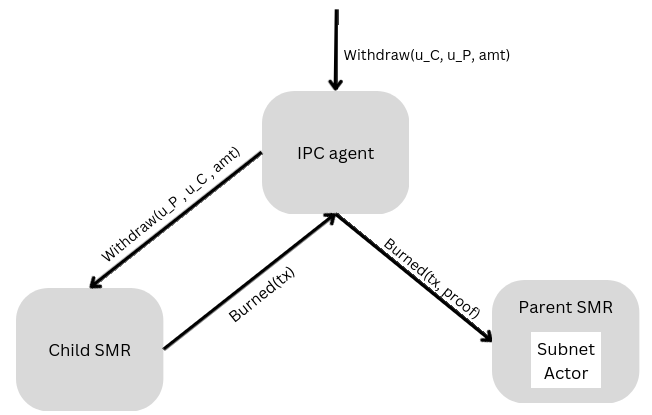
\includegraphics[width=\textwidth]{withdrawal}
     \caption{Events produced and consumed during a withdrawal.}
     \label{fig:withdrawal}
 \end{figure}
\begin{algorithm}[H]
\footnotesize
\caption{Withdraw operation}\label{alg:down}
  \DontPrintSemicolon
  \SetKwFunction{FMain}{Global}
  \SetKwProg{Pn}{Function}{:}{\KwRet}
  \SetKwInOut{Input}{input}
  \SetKwProg{Component}{$\blacktriangleright$ \bf}{:}{\KwRet}
  \SetKwFor{UponKW}{upon}{do}{fintq}
  % \Input{user~$\user$, amount~$\fil$, transaction \txnf}
   \Input{\src account in child, \dest account in parent, $\fil$ amount of coins}
   \Component{IPC agent}{
        submit $\tx=\textit{Withdraw}(\src, \fil, \dest)$ to child \smr\;
  }
   %
   \Component{Child \smr replica}{
   \UponKW{$\tx = \textit{Withdraw}(\src, \fil, \dest)$}{
    deduct $\fil$ from \src account at child \tcp{``burns" \fil in child}
    notify agent \texttt{Burned}(\tx)
   }
  }
  \Component{IPC agent}{
    \UponKW{notification of \texttt{Burned}(\tx) from child \smr replica}{
    
        create \prf that \tx is final at child \smr \tcp*[r]{see Sec.~? for details}
        submit $\tx'=\texttt{Burned}\left(\tx, \prf \right)$  to parent \smr replica
     }
  }
  \Component{parent \smr replica}{
    \UponKW{$\tx'=\texttt{Burned}\left(\tx, \prf \right)$}{
        assert \sa.\verifyGfinal{\prf}{\tx}\;
        move \fil coins from \sa.accounts[\src] to \dest
     }
  }
   
%    \Component{Child SMR}{
%    [\tx submitted by user, proposed, written]\\
%    \UponKW{\txnf written in Child SMR}{
%     decrease user fund's by $\fil$\\
%     Send \texttt{ChildWithdrawn(\tx, [$proof$])} to IPC agent \tcp*[r]{notify IPC agent}
%    }
%   }
%   \Component{IPC agent}{
%     \UponKW{\texttt{ChildWithdrawn(\tx, [$proof$])} notified by Child SMR}{
%     \If{$proof=$ \textbf{nil}}{
%          $proof \gets $\textit{generateProofOfGlobalFinality(\tx,...)} \tcp*[r]{Necessary steps for \tx to be ready to be submitted to Parent SMR}
%      }
%      \texttt{ChildWithdrawn(\tx, $proof$)} to parent SMR \tcp*[r]{Submit to parent}
%      }
%     \UponKW{\arp{State updated after Withdrawal}}{ \tcp*[r]{Notified when parents update state}
%       \arp{Check child subnet rules are still satisfied, remedy/close otherwise?}
%     }
%   }
%   \Component{Parent SMR}{
%   \UponKW{\texttt{ChildWithdrawn(\tx, $proof$)} submitted by IPC agent}{
%       \If{\sa.\verifyGfinal{\tx}{\prf}}{
%            [tx submitted by IPC agent, proposed, written]\\
%            \UponKW{\txnf written in Parent SMR}{
%                 reduce $\fil$ amount for user $\user$ in SA\\
%                 Parent SMR notifies IPC agent
%             }
%       }
%   }
% }
\end{algorithm}
\subsection{Enhanced Functionality}
\label{enhancedFunc}
\arp{From here below we need to add the gateway actor and refine the functionality, leave out till round of feedback for GW}
We show here a list of desirable functionalities that build upon the basic withdrawals and deposits.
\subsubsection{Checkpointing} A checkpoint contains a representation of the updated state of the child SMR system to be included in the parent SMR system. A checkpoint can be triggered by predefined events (i.e. periodically after a number of state updates, triggered by a specific user or set of users, etc.). As such, the checkpoint functionality may or may not be triggered by a user request on the child SMR. A checkpoint is performed as follows: 
\begin{enumerate}
\item If the predefined checkpoint trigger is met, then the IPC agent queries the child SMR replica for the updated state to be represented in this checkpoint.
\item The IPC agent creates a proof \prf that this updated state of the child SMR system is final, possibly compressing its representation of the state.
\item The IPC agent submits a transaction $\tx'=\texttt{Checkpoint}\left(\textit{state}, \prf \right)$ to the parent SMR replica
 \item Upon ordering $tx'$, the replicated logic of the parent SMR system updates the state of the SA according to the checkpoint state, if necessary.
\end{enumerate}

\begin{figure}[h]
     \centering
     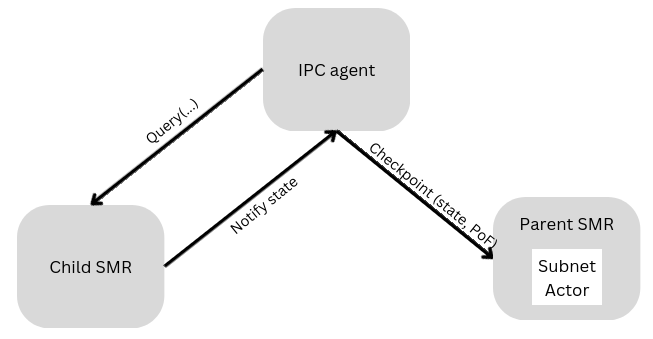
\includegraphics[width=\textwidth]{checkpoint.png}
     \caption{Events produced and consumed by the checkpointing functionality.}
     \label{fig:chkp}
 \end{figure}
\begin{algorithm}[H]
\footnotesize
\caption{Checkpoint operation}\label{alg:down}
  \DontPrintSemicolon
  \SetKwFunction{FMain}{Global}
  \SetKwProg{Pn}{Function}{:}{\KwRet}
  \SetKwInOut{Input}{input}
  \SetKwProg{Component}{$\blacktriangleright$ \bf}{:}{\KwRet}
  \SetKwFor{UponKW}{upon}{do}{fintq}
   \Component{IPC agent}{
        \If{trigger for checkpoint}{
            \textit{state} $\gets$ query the child \smr replica for the state\;
            create \prf that \textit{state} is final at child \tcp*[r]{Possibly compress \textit{state}}
        }
        submit $\tx'=\texttt{Checkpoint}\left(\textit{state}, \prf \right)$  to parent \smr replica
  }
  \Component{parent \smr replica}{
    \UponKW{$\tx'=\texttt{Checkpoint}\left(\textit{state}, \prf \right)$}{
        assert \sa.\verifyGfinal{\prf}{\textit{state}}\;
        $\sa.\textit{latestCheckpoint} \gets \textit{state}$
     }
  }
  
  % \Input{[User's checkpoint request]}
  % \Component{Child SMR}{
  %    \UponKW{State updated [ \textbar User's checkpoint request]}{ 
  %       [Write checkpoint request if any]\\
  %      Send \texttt{StateUpdated($st$)} to IPC agent \tcp*[r]{Notify IPC agent}
  %    }
  % }
  % \Component{IPC agent}{
  %   \UponKW{\texttt{StateUpdated($st$)} notified by child SMR}{
  %       \If{\texttt{SatisfiesCheckpointCondition($st$)}}{
  %          Create checkpoint \chkp\\
  %           $proof \gets $\textit{generateProofOfGlobalFinality($st$,...)} \tcp*[r]{Necessary steps for \tx to be ready to be submitted to Parent SMR}
  %           Submit \texttt{SubmitCheckpoint(\chkp)} to parent SMR
  %           }
  %       }
  % }
  % \Component{Parent SMR}{
  %     \UponKW{\texttt{SubmitCheckpoint(\chkp)} submitted by IPC agent}{
  %        [\chkp proposed, written]\\
  %        Refund fee to submitter \tcp*[r]{refund at parent for simplicity}
  %     }
  % }
\end{algorithm}

\subsubsection{Slashing} 
\guy{This section is immature for review (even a preliminary one)}\\
We show here the events produced and consumed by the slashing functionality. Given specific misbehavior from participants that is identified as Proofs of Fraud (PoFs), e.g.
gathering signed equivocating messages, the child SMR reports the PoFs to the IPC agent, which immediately forwards a slash a request to the parent SMR. \arp{Extend with need to verify if child SMR can continue, needs to remedy its depleted collateral or should be killed with latest checkpoint/state update}.
\begin{figure}[h]
     \centering
     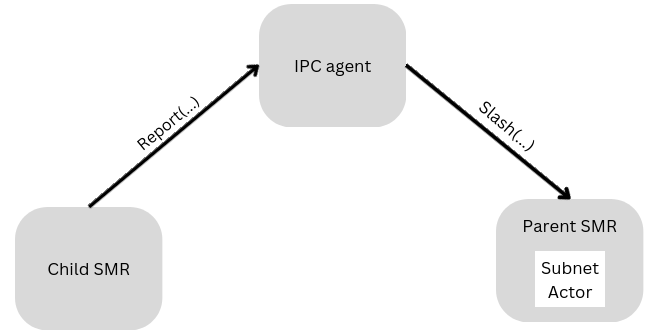
\includegraphics[width=\textwidth]{slash}
     \caption{Events produced and consumed by the slashing functionality.}
     \label{fig:report}
 \end{figure}\\

\begin{algorithm}[H]
\footnotesize
\caption{Slash Functionality}\label{alg:down}
  \DontPrintSemicolon
  \SetKwFunction{FMain}{Global}
  \SetKwProg{Pn}{Function}{:}{\KwRet}
  \SetKwInOut{Input}{input}
  \SetKwProg{Component}{$\blacktriangleright$ \bf}{:}{\KwRet}
  \SetKwFor{UponKW}{upon}{do}{fintq}
  \Input{-}
  \Component{Child SMR}{
     \UponKW{Proofs of fraud \pofs generated}{
       Notify \report to IPC agent
     }
  }
  \Component{IPC agent}{
    \UponKW{\report notified by child SMR}{
        Submit \slashop to parent SMR
    }
    \UponKW{\arp{State updated after slashing}}{
      \arp{Check child SMR rules are still satisfied, remedy/close otherwise?}
    }
  }
  \Component{Parent SMR}{
        \UponKW{\slashop submitted by IPC agent}{
         Update SA state slashing/excluding participants
         Notify SA update to IPC agent
        }
  }
\end{algorithm}


\subsubsection{\postoffice}
The \postoffice functionality is an inter-subnet transaction service. The main motivation for this functionality comes from a ``potential clients" request: enable a \dapp in one subnet to interact with a \dapp in a different subnet.\\
\guy{Edge case: a leaf subnet does not have a \sa and, therefore, no \postoffice. We can consider removing the \postoffice functionality from the \sa and to deploy it as an independent \dapp that will appear only once per subnet. In this case, it needs permissions to call \sa.\verifyGfinal{\tx}{\prf} function.}

\begin{algorithm}[H]
\footnotesize
\caption{\postoffice Functionality}\label{alg:po}
  \DontPrintSemicolon
  \SetKwFunction{FPropagate}{propagate}
  \SetKwProg{Pn}{Function}{:}{\KwRet}
  \SetKwInOut{Input}{input}
  \SetKwProg{Component}{$\blacktriangleright$ \bf}{:}{\KwRet}
  \SetKwProg{Empty}{\bf}{:}{\KwRet}
  \SetKwFor{UponKW}{upon}{do}{fintq}
  \Input{$\tx = \langle \data, \src, \dest, \prf \rangle$}
  \Component{\sa.\postoffice}{
     \UponKW{\postoffice.\propagate(\tx) }{
       \Case{\dest in current subnet}{
            \postoffice.\propagate\textit{HERE}(\tx)
       }
       \Case{\dest requires going up the tree}{
            \postoffice.\propagate\textit{UP}(\tx)
       }
       \Case{\dest requires going down the tree}{
            \postoffice.\propagate\textit{DOWN}(\tx)
       }
     }
     \UponKW{\postoffice.\propagate\textit{UP}(\tx) }{
       \If{\src not from this subnet}{
            assert(\sa.\verifyGfinal{\tx}{\prf})\;
       }
       \src.\textit{append(\sa's subnet id)}\;
       emit event \postoffice.UP$\langle \data, \src, \dest \rangle$
     }
     \tcp{\propagate\textit{DOWN}(\tx) is analogous to \propagate\textit{UP}(\tx)}
     \tcp{\propagate\textit{HERE}(\tx) is trivial}
  }
  \Component{parent \smr process}{
     \UponKW{event \postoffice.UP$\langle \data, \src, \dest \rangle$}{
        $\tx \gets \langle \data, \src, \dest \rangle$\;
        notify agent on \postoffice.UP(\tx)
     }
  }
  \Component{IPC agent}{
    \UponKW{notification of \propagate\textit{UP}(\tx) from child \smr}{
        create \prf that \textit{UP}(\tx) is final at child \smr\;
        $\tx_\textit{new}\gets\langle \textit{UP}(\tx), \prf \rangle$\;
        submit \sa.\postoffice.\propagate($\tx_\textit{new}$) to parent \smr
    }   
}
\end{algorithm}
\subsubsection{Atomic Execution}
TODO Discuss in Lanzarote?


\subsection{Future}
\label{sec:future}
 % - Implementations/templates
 %  - Different types and trade-offs of checkpoint triggers 
 %    - Periodically: time, #blocks, #withdrawn, etc.
 %    - At request: (this one is not governance funded)
 %    - Combinations of these 
 %    - Slashing functions
 %    - Atomic execution types?
 \section{An Instance of IPC}
 \label{sec:impl-tmpl}
 Here we describe the particular choices implemented by the Consensus Lab team.

The current implementation considers Filecoin as the root subnet\guy{I wrote it but I'm not sure this is the case...}, and Trantor as child subnets. For our interest it is important to note that Trantor is a BFT consensus protocol with immediate finality, and Filecoin is a longest chain style protocol with probabilistic finality. Therefore, as a \prf that a child subnet finalized a state we use a multisig on that state, the multisig must correspond to more than 2/3 of the child's validators voting rights as reflected by \sa at the time.%
\footnote{A next step in the implementation road-map is to offer a threshold signature mechanism instead of using a multisig. For now, multisigs serve the purpose of an MVP implementation.}
To verify the finality of a state at the parent, we use the fact that a participant has view in to a version of the parent blockchain (through its local parent replica process). In this case, \prf contains the block height~$h$ (and pointer to that block) at the parent subnet. A child replica then asserts with its parent that the state is final by checking with its local version of the parent blockchain at height~$h$. If the the local version at the parent replica did not reach height~$h$ yet, the child replica considers the state non-final/non-valid currently and checks again when the parent reaches height~$h$.
\section{Verifying the Finality of \tx{tx}}
\arp{I think this section should contain much more than this (but that perhaps this section does not follow our timelines for document completion (more of a complement of the document). Particular content here imo: Analysis for improvements wrt reference implementations (i.e. threshold signatures instead of everyone submitting checkpoints, governance account instead of no incentives, etc.); and Comprehensive list of different approaches for functionality/functions (like we had in the legacy document).}\guy{Agreed}
\label{sec:finality}
A main ingredient in any \ipcFull implementation is the creation and verification of a finality proof for a given \tx{tx} in some subnet. In the previous sections we left these functions opaque. For example, \sa.\verifyGfinal{\tx{tx}}{\prf} was used by the parent replica to verify the finality at the child subnet of \tx{tx}. The creation of \prf and the verification method at the child replica (for transactions of that occur at the parent subnet), are only hinted by plain text. There are multiple ways to implement these functionalities, each with its own trade-offs. Below we propose several such implementations.

 % - Components and their Interfaces
 %   - Parent subnet node
 %   - Child subnet node
 %   - IPC module
 %   - Subnet actor
 % - IPC Functionality
 %  - Minimum required per subnet
 %    - Withdrawal/Deposits Interfaces
 %    - Other Operations? (Propagate?)
 %  - Enhancements
 %    - Checkpointing interfaces
 %    - Propagate
 %    - Reporting/Slashing interfaces
 %    - Atomic execution/swap, IBC-like bridges
 %  - Future stuff (google docs?)
 %    - Withdrawal at ancestor (skip parent(s)) (with timeout) etc.
 % - Implementations/templates
 %  - Different types and trade-offs of checkpoint triggers 
 %    - Periodically: time, #blocks, #withdrawn, etc.
 %    - At request: (this one is not governance funded)
 %    - Combinations of these 
 %    - Slashing functions
 %    - Atomic execution types?
 
% ----------------------------------------------------------------
% ----------------------------------------------------------------

%%
%% The next two lines define the bibliography style to be used, and
%% the bibliography file.
\bibliographystyle{plain}
\bibliography{bibliography}

%%
%% If your work has an appendix, this is the place to put it.
\appendix
% ----------------------------------------------------------------
% ----------------------------------------------------------------
\newpage
% \section{Glossary}
\label{sec:gls}
\TODO{(Marko)Add IPC Glossary~\cite{glossary} here and move most of model down here}


% \input{sections/algorithm.tex}
% \input{sections/QvW.tex}
% \input{sections/Yao.tex}
% ----------------------------------------------------------------
% ----------------------------------------------------------------

%%%%%%%%%%%%%%%%%%%%%%%%%%%%%%%%%%%%%%%%%%%%%%%%%%%%%%%%%%%%%%%%%%
%%%%%%%%%%%%%%%%%%%%%%%%%%%%%%%%%%%%%%%%%%%%%%%%%%%%%%%%%%%%%%%%%%

\end{document}
\endinput
%%
%% End of file 
